%%%%%%%%%%%%%%%%%%%%%%%%%%%%%%%%%%%%%%%%%%%%%%%%%%%%%%%%%%%%%%%%%%%%%%%%%%%
%
% Template for a LaTex article in English.
%
%%%%%%%%%%%%%%%%%%%%%%%%%%%%%%%%%%%%%%%%%%%%%%%%%%%%%%%%%%%%%%%%%%%%%%%%%%%

\documentclass[12pt]{article}
\usepackage{times}
%\usepackage{arial}
%\usepackage{helvet}
%\usepackage{uarial}

% AMS packages:
\usepackage{amsmath, amsthm, amsfonts}

\usepackage[top=1in, bottom=0.8in, left=0.8in, right=0.8in]{geometry}
\usepackage{graphicx}  
\usepackage{float}
\usepackage{fontenc}
\usepackage{sidecap}
\usepackage{parskip}
\usepackage{siunitx}
\usepackage{hyperref}
\usepackage{tikz}

\setlength{\parskip}{1em}

\linespread{1.2}

% Shortcuts.
% One can define new commands to shorten frequently used
% constructions. As an example, this defines the R and Z used
% for the real and integer numbers.
%-----------------------------------------------------------------
\def\RR{\mathbb{R}}
\def\ZZ{\mathbb{Z}}

% Similarly, one can define commands that take arguments. In this
% example we define a command for the absolute value.
% -----------------------------------------------------------------
\newcommand{\abs}[1]{\left\vert#1\right\vert}

% Operators
% New operators must defined as such to have them typeset
% correctly. As an example we define the Jacobian:
% -----------------------------------------------------------------
\DeclareMathOperator{\Jac}{Jac}

%-----------------------------------------------------------------
\title{Residential Home Energy Consumption Survey}
%\author{Amir A. Aliabadi}

\begin{document}
\maketitle

\begin{center}
This document is typeset using \LaTeX

\large
\textbf{Did you know that buildings are responsible for 40\% of global energy use?}
\normalsize
\end{center}

\begin{figure}[H]
\begin{center}
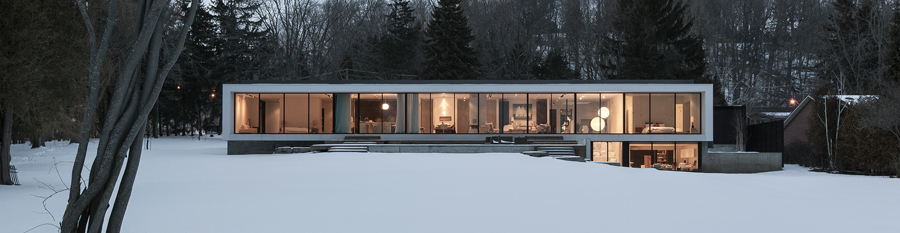
\includegraphics[width=\textwidth]{Figures/OppositeHouseNarrow.png} 
\caption{Opposite House, designed by Atelier RZLBD, Toronto, Canada}
\label{OppositeHouseNarrow}
\vspace{-0.5cm}
\end{center}
\end{figure}

In an effort to combat climate change, this survey attempts to collect data for academic research on building energy consumption in Canada and the United States. Data will be used to understand building performance, develop prediction and design models, and lead innovation to reduce building energy consumption. By participation in this survey, your privacy will be protected. To protect individual's data, information will be collected as anonymous and only reported in aggregate form, i.e. by combining large sets of data. This study is organized by Amir A. Aliabadi from Environmental Engineering at the University of Guelph. Please complete this form and email it to \href{mailto:aliabadi@uoguelph.ca}{aliabadi@uoguelph.ca}. To access the form visit: 

\url{www.aaa-scientists.com/ResidentialHomeEnergyConsumptionSurvey.pdf}

\begin{figure}

\includegraphics[height=0.1\textwidth]{Figures/AIR Logo Text}

\includegraphics[height=0.1\textwidth]{Figures/qrcode_42723388_365d17d4489069d364e3c3dad5b734c8}
\end{figure}

\pagebreak

\section{Basic Information About Your Residential Home}


\begin{Form}
Q1. Your postal code (Example: N1G 1X9 or 02119):	
\TextField[name=Q1_1, width=5em, height=1em]{}
	
Q2. Type of your residential home:
\ChoiceMenu[combo, name=Q2_1,width=8cm,charsize=10pt,default=Single-detached house]{}
{Single-detached house, Semi-detached house, Row house, Apartment in a building with less than 5 storeys, Apartment in a building with more than 5 storeys, Other} \\	
\TextField[name=Q2_2, width=38em, height=1em]{Other :}

Q3. Number of people living in your home:
\ChoiceMenu[combo, name=Q3_1,width=3cm,charsize=10pt,default=4]{}
{1,2,3,4,5,6,7,8,9,10}

Q4. What is the approximate footprint area of your residential home? For multi-storey buildings, the footprint area is only associated with one storey of the building; please exclude garages, yards, and other
spaces that are not heated or cooled: 
\ChoiceMenu[combo, name=Q4_1,width=6.5cm,charsize=10pt,default=Small: about 100 m2 or 1000 ft2]{}
{Tiny: about 50 m2 or 500 ft2, Small: about 100 m2 or 1000 ft2, Medium: about 200 m2 or 2000 ft2, Large: about 300 m2 or 3000 ft2, Supersize: about 400 m2 or 4000 ft2, Other}\\
\TextField[name=Q4_2, width=38em, height=1em]{Other:}
\end{Form}

\begin{Form}
Q5. How many storeys in your residential home are heated and/or cooled? \\ 
\ChoiceMenu[combo, name=Q5_1, width=10cm, charsize=10pt, default=1 (flat apartment or bungalow house with possibly a basement)]{}
{1 (flat apartment or bungalow house with possibly a basement), 2 (back-split apartment or house with possibly a basement), 3 (two-level apartment or house with possibly a basement), 4 (three-level apartment or house with possibly a basement), 5 (four-level apartment or house with possibly a basement), Other}\\
\TextField[name=Q5_2, width=38em, height=1em]{Other:}	
\end{Form}

\begin{Form}
Q6. Type of space heating system:
\ChoiceMenu[combo, name=Q6_1, width=8cm, charsize=10pt, default=Natural gas furnace (most common)]{}
{Natural gas furnace (most common), Heat pump powered by electricity (used in moderate climates), Baseboard powered by electricity or electric heaters, I don't have a space heating system, Other}\\
\TextField[name=Q6_2, width=38em, height=1em]{Other:}
\end{Form}


\begin{Form}
Q7. Type of space cooling system:
\ChoiceMenu[combo, name=Q7_1, width=7cm, charsize=10pt, default=Air conditioning: vapor compression (most common)]{}
{Air conditioning: vapor compression (most common), Evaporative cooling system (used in dry climates), I don't have a space cooling system, Other}\\
\TextField[name=Q7_2, width=38em, height=1em]{Other:}
\end{Form}


\begin{Form}
Q8. Type of water heating system: 
\ChoiceMenu[combo, name=Q8_1, width=4cm, charsize=10pt, default=Natural gas water heater (most common)]{}
{Natural gas water heater (most common), Electric water heater (less common), I don't have a water heating system, Other }\\
\TextField[name=Q8_2, width=38em, height=1em]{Other:}	
\end{Form}

\begin{Form}
Q9. Type of stove/oven system: 
\ChoiceMenu[combo, name=Q9_1, width=4cm, charsize=10pt, default=Natural gas]{}
{Natural gas, Electric, Both natural gas and electric, Other }\\
\TextField[name=Q9_2, width=38em, height=1em]{Other:}	
\end{Form}


\begin{Form}
Q10. Which one of the uncommon devices below depend on substantial amount of energy in your home (choose as many as may apply)?\\
\CheckBox[name=Q10_1, width=1em, height=0.8em]{1} Electric car charged by electricity \\
\CheckBox[name=Q10_2, width=1em, height=0.8em]{2} Fire place powered by natural gas \\
\CheckBox[name=Q10_3, width=1em, height=0.8em]{3} Swimming pool, sauna, etc. \\
\CheckBox[name=Q10_4, width=1em, height=0.8em]{4} No uncommon devices \\
\TextField[name=Q10_5, width=38em, height=1em]{Other:}
\end{Form}
	
\begin{Form}
Q11. Approximately when was your residential home built?
\ChoiceMenu[combo, name=Q11_1, width=3cm, charsize=10pt, default=After 2000s]{}
{Before 1950s, Between 1950s and 2000s, After 2000s, I don't know}
\end{Form}

\begin{Form}
Q12. When was your residential home retrofitted for energy efficiency?
\ChoiceMenu[combo, name=Q12_1, width=3cm, charsize=10pt, default=After 2000s]{}
{Before 1950s, Between 1950s and 2000s, After 2000s, Never, I don't know}
\end{Form}

\begin{Form}
Q13. If your home has been retrofitted for energy efficiency, click on all the features that apply to your home. Describe any specifics of the system components (e.g. the size of your photovoltaic panels, etc.)?

\CheckBox[name=Q13_1, width=1em, height=0.8em]{1} My home was air-leak tested and now it is leak-proof \\
\TextField[name=Q13_2, width=37.5em, height=1em]{Specifics:}
	
\CheckBox[name=Q13_3, width=1em, height=0.8em]{2} I replaced my windows with energy efficient windows (e.g. double or tripple-layer)\\
\TextField[name=Q13_4, width=37.5em, height=1em]{Specifics:}
	
\CheckBox[name=Q13_5, width=1em, height=0.8em]{3} I installed a high efficiency furnace \\ 
\TextField[name=Q13_6, width=37.5em, height=1em]{Specifics:}
	
\CheckBox[name=Q13_7, width=1em, height=0.8em]{4} I increased the thermal insulation of my building envelop (e.g. increase R-value, foam spray under roof, etc.) \\
\TextField[name=Q13_8, width=37.5em, height=1em]{Specifics:}

\CheckBox[name=Q13_9, width=1em, height=0.8em]{5} I installed a photovoltaic system \\
\TextField[name=Q13_10, width=37.5em, height=1em]{Specifics:}
	
\CheckBox[name=Q13_11, width=1em, height=0.8em]{6} I installed a heat pump for home heating \\
\TextField[name=Q13_12, width=37.5em, height=1em]{Specifics:}
	
\CheckBox[name=Q13_13, width=1em, height=0.8em]{7} I installed a solar thermal collector \\
\TextField[name=Q13_14, width=37.5em, height=1em]{Specifics:}
	
\CheckBox[name=Q13_15, width=1em, height=0.8em]{8} I installed a thermal energy storage system \\
\TextField[name=Q13_16, width=37.5em, height=1em]{Specifics:}
	
\CheckBox[name=Q13_17, width=1em, height=0.8em]{9} I have installed a green roof \\
\TextField[name=Q13_18, width=37.5em, height=1em]{Specifics:}
	
\CheckBox[name=Q13_19, width=1em, height=0.8em]{10} I have installed other systems not described above \\
\TextField[name=Q13_20, width=37.5em, height=1em]{Specifics:}
\end{Form}

\pagebreak

\section{Natural Gas or Other Fuel Consumption Data}

Q14. Would you share your natural gas or other fuel consumption data?

\begin{itemize}
\item Yes, I will fill the table below to indicate my natural gas (or other fuel) consumption. Note: the entries below can be populated by referring to your natural gas (or other fuel) bills (e.g. Figure \ref{Enbridge} below). Please fill up to 12 entries. It is recommended to consider bills for at least 1 full year of natural gas (of other fuel) consumption. Your bills should come from the utility company in your region, such as Enbridge. If you have consumption data for less than 1 full year, that is still fine.
\end{itemize}

\begin{figure}[H]
\begin{center}
\begin{tikzpicture}
\pgftext{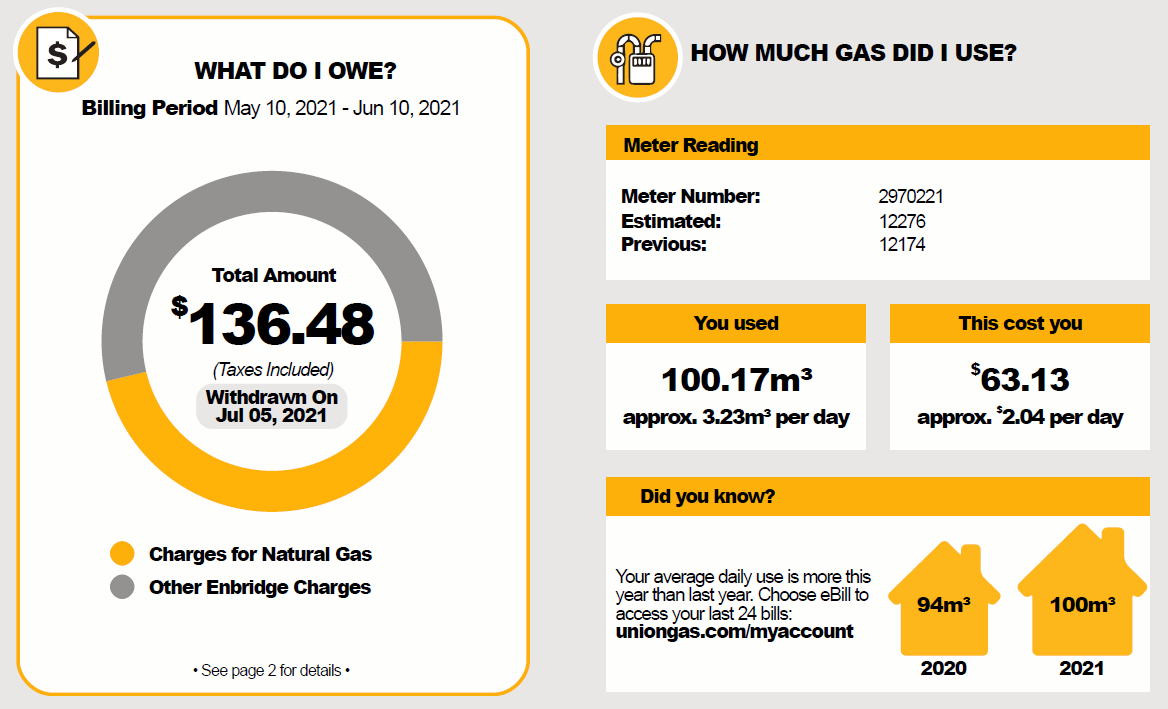
\includegraphics[width=\textwidth]{Figures/Enbridge.png}} at (0,0);
\draw [-, thick, draw=red] (-8,3.3) rectangle (-1.3,4); 
\draw [-, thick, draw=red] (0.1,-1.7) rectangle (4.5,1);
\draw [-, thick, draw=red, fill=red] (4,2.2) rectangle (6,2.5);
\end{tikzpicture}
\caption{Sample natural gas bill with billing period (May 10, 2021 - Jun 10, 2021) and consumption (100.17 \SI{}{m^3}) boxed in red}
\label{Enbridge}
\end{center}
\end{figure}

\pagebreak

Q15. Provide Information on up to 12 bills: consumption in cubic meters (\SI{}{m^3})

\begin{Form}
Bill 01: 
\TextField[name=Q15_1_1, width=2em, height=0.8em]{Start YYYY} \TextField[name=Q15_1_2, width=1.5em, height=0.8em]{MM}
\TextField[name=Q15_1_3, width=1.5em, height=0.8em]{DD} \TextField[name=Q15_1_4, width=2em, height=0.8em]{End YYYY} \TextField[name=Q15_1_5, width=1.5em, height=0.8em]{MM}
\TextField[name=Q15_1_6, width=1.5em, height=0.8em]{DD} \TextField[name=Q15_1_7, width=3em, height=0.8em]{Consumption}

Bill 02: 
\TextField[name=Q15_2_1, width=2em, height=0.8em]{Start YYYY} \TextField[name=Q15_2_2, width=1.5em, height=0.8em]{MM}
\TextField[name=Q15_2_3, width=1.5em, height=0.8em]{DD} \TextField[name=Q15_2_4, width=2em, height=0.8em]{End YYYY} \TextField[name=Q15_2_5, width=1.5em, height=0.8em]{MM}
\TextField[name=Q15_2_6, width=1.5em, height=0.8em]{DD} \TextField[name=Q15_2_7, width=3em, height=0.8em]{Consumption}

Bill 03: 
\TextField[name=Q15_3_1, width=2em, height=0.8em]{Start YYYY} \TextField[name=Q15_3_2, width=1.5em, height=0.8em]{MM}
\TextField[name=Q15_3_3, width=1.5em, height=0.8em]{DD} \TextField[name=Q15_3_4, width=2em, height=0.8em]{End YYYY} \TextField[name=Q15_3_5, width=1.5em, height=0.8em]{MM}
\TextField[name=Q15_3_6, width=1.5em, height=0.8em]{DD} \TextField[name=Q15_3_7, width=3em, height=0.8em]{Consumption}

Bill 04: 
\TextField[name=Q15_4_1, width=2em, height=0.8em]{Start YYYY} \TextField[name=Q15_4_2, width=1.5em, height=0.8em]{MM}
\TextField[name=Q15_4_3, width=1.5em, height=0.8em]{DD} \TextField[name=Q15_4_4, width=2em, height=0.8em]{End YYYY} \TextField[name=Q15_4_5, width=1.5em, height=0.8em]{MM}
\TextField[name=Q15_4_6, width=1.5em, height=0.8em]{DD} \TextField[name=Q15_4_7, width=3em, height=0.8em]{Consumption}

Bill 05: 
\TextField[name=Q15_5_1, width=2em, height=0.8em]{Start YYYY} \TextField[name=Q15_5_2, width=1.5em, height=0.8em]{MM}
\TextField[name=Q15_5_3, width=1.5em, height=0.8em]{DD} \TextField[name=Q15_5_4, width=2em, height=0.8em]{End YYYY} \TextField[name=Q15_5_5, width=1.5em, height=0.8em]{MM}
\TextField[name=Q15_5_6, width=1.5em, height=0.8em]{DD} \TextField[name=Q15_5_7, width=3em, height=0.8em]{Consumption}

Bill 06: 
\TextField[name=Q15_6_1, width=2em, height=0.8em]{Start YYYY} \TextField[name=Q15_6_2, width=1.5em, height=0.8em]{MM}
\TextField[name=Q15_6_3, width=1.5em, height=0.8em]{DD} \TextField[name=Q15_6_4, width=2em, height=0.8em]{End YYYY} \TextField[name=Q15_6_5, width=1.5em, height=0.8em]{MM}
\TextField[name=Q15_6_6, width=1.5em, height=0.8em]{DD} \TextField[name=Q15_6_7, width=3em, height=0.8em]{Consumption}

Bill 07: 
\TextField[name=Q15_7_1, width=2em, height=0.8em]{Start YYYY} \TextField[name=Q15_7_2, width=1.5em, height=0.8em]{MM}
\TextField[name=Q15_7_3, width=1.5em, height=0.8em]{DD} \TextField[name=Q15_7_4, width=2em, height=0.8em]{End YYYY} \TextField[name=Q15_7_5, width=1.5em, height=0.8em]{MM}
\TextField[name=Q15_7_6, width=1.5em, height=0.8em]{DD} \TextField[name=Q15_7_7, width=3em, height=0.8em]{Consumption}

Bill 08: 
\TextField[name=Q15_8_1, width=2em, height=0.8em]{Start YYYY} \TextField[name=Q15_8_2, width=1.5em, height=0.8em]{MM}
\TextField[name=Q15_8_3, width=1.5em, height=0.8em]{DD} \TextField[name=Q15_8_4, width=2em, height=0.8em]{End YYYY} \TextField[name=Q15_8_5, width=1.5em, height=0.8em]{MM}
\TextField[name=Q15_8_6, width=1.5em, height=0.8em]{DD} \TextField[name=Q15_8_7, width=3em, height=0.8em]{Consumption}

Bill 09: 
\TextField[name=Q15_9_1, width=2em, height=0.8em]{Start YYYY} \TextField[name=Q15_9_2, width=1.5em, height=0.8em]{MM}
\TextField[name=Q15_9_3, width=1.5em, height=0.8em]{DD} \TextField[name=Q15_9_4, width=2em, height=0.8em]{End YYYY} \TextField[name=Q15_9_5, width=1.5em, height=0.8em]{MM}
\TextField[name=Q15_9_6, width=1.5em, height=0.8em]{DD} \TextField[name=Q15_9_7, width=3em, height=0.8em]{Consumption}

Bill 10: 
\TextField[name=Q15_10_1, width=2em, height=0.8em]{Start YYYY} \TextField[name=Q15_10_2, width=1.5em, height=0.8em]{MM}
\TextField[name=Q15_10_3, width=1.5em, height=0.8em]{DD} \TextField[name=Q15_10_4, width=2em, height=0.8em]{End YYYY} \TextField[name=Q15_10_5, width=1.5em, height=0.8em]{MM}
\TextField[name=Q15_10_6, width=1.5em, height=0.8em]{DD} \TextField[name=Q15_10_7, width=3em, height=0.8em]{Consumption}

Bill 11: 
\TextField[name=Q15_11_1, width=2em, height=0.8em]{Start YYYY} \TextField[name=Q15_11_2, width=1.5em, height=0.8em]{MM}
\TextField[name=Q15_11_3, width=1.5em, height=0.8em]{DD} \TextField[name=Q15_11_4, width=2em, height=0.8em]{End YYYY} \TextField[name=Q15_11_5, width=1.5em, height=0.8em]{MM}
\TextField[name=Q15_11_6, width=1.5em, height=0.8em]{DD} \TextField[name=Q15_11_7, width=3em, height=0.8em]{Consumption}

Bill 12: 
\TextField[name=Q15_12_1, width=2em, height=0.8em]{Start YYYY} \TextField[name=Q15_12_2, width=1.5em, height=0.8em]{MM}
\TextField[name=Q15_12_3, width=1.5em, height=0.8em]{DD} \TextField[name=Q15_12_4, width=2em, height=0.8em]{End YYYY} \TextField[name=Q15_12_5, width=1.5em, height=0.8em]{MM}
\TextField[name=Q15_12_6, width=1.5em, height=0.8em]{DD} \TextField[name=Q15_12_7, width=3em, height=0.8em]{Consumption}

\end{Form}

\pagebreak

\section{Electricity Consumption Data}

Q16. Would you share your electricity consumption data?

\begin{itemize}
\item Yes, I will fill the table below to indicate my electricity consumption. Note: the entries below can be populated by referring to your electricity bills (e.g. Figure \ref{Hydro} below). Please fill up to 12 entries. It is recommended to consider bills for at least 1 full year of electricity consumption. Your bills should come from the utility company in your region, such as Toronto Hydro. If you have consumption data for less than 1 full year, that is still fine.
\end{itemize}

\begin{figure}[H]
\begin{center}
\begin{tikzpicture}
\pgftext{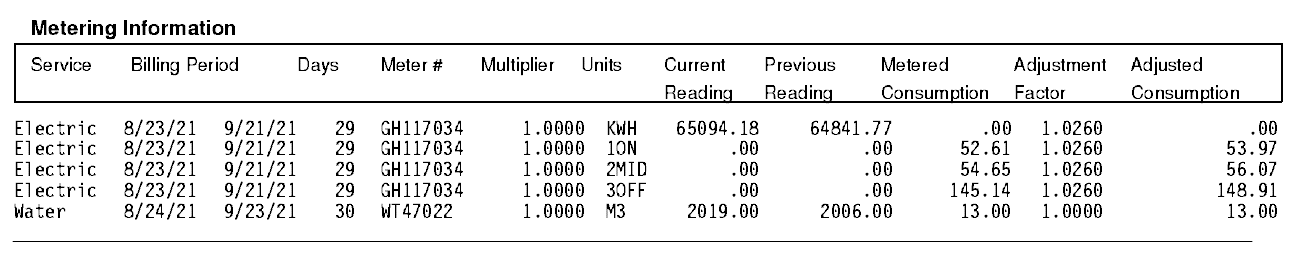
\includegraphics[width=\textwidth]{Figures/Hydro.png}} at (0,0);
% \draw [-, thick, draw=red] (-7.3,-0.9) rectangle (-4.6,-0.1); 
% \draw [-, thick, draw=red] (7.4,-0.9) rectangle (8.7,-0.1);
% \draw [-, thick, draw=red, fill=red] (-3.7,-1.2) rectangle (-2.0,0.2);;
\end{tikzpicture}
\caption{Sample electricity bill with billing period (8/23/21 to 9/21/21) and consumption ($53.97 + 56.07 + 148.91 = 258.95$ \SI{}{kW-hr}) boxed in red; in this example electricity price varies according to time of year and day in three brackets; we consider adding all the consumptions together}
\label{Hydro}
\end{center}
\end{figure}

\pagebreak

Q17. Provide Information on up to 12 bills: consumption in kilo Watt hours (kW-hr); please note that in some regions the electricity price varies according to time of year and day. In such cases, simply report the total electricity used in the billing cycle by adding all the consumptions together.

\begin{Form}
Bill 01: 
\TextField[name=Q17_1_1, width=2em, height=0.8em]{Start YYYY} \TextField[name=Q17_1_2, width=1.5em, height=0.8em]{MM}
\TextField[name=Q17_1_3, width=1.5em, height=0.8em]{DD} \TextField[name=Q17_1_4, width=2em, height=0.8em]{End YYYY} \TextField[name=Q17_1_5, width=1.5em, height=0.8em]{MM}
\TextField[name=Q17_1_6, width=1.5em, height=0.8em]{DD} \TextField[name=Q17_1_7, width=3em, height=0.8em]{Consumption}
	
Bill 02: 
\TextField[name=Q17_2_1, width=2em, height=0.8em]{Start YYYY} \TextField[name=Q17_2_2, width=1.5em, height=0.8em]{MM}
\TextField[name=Q17_2_3, width=1.5em, height=0.8em]{DD} \TextField[name=Q17_2_4, width=2em, height=0.8em]{End YYYY} \TextField[name=Q17_2_5, width=1.5em, height=0.8em]{MM}
\TextField[name=Q17_2_6, width=1.5em, height=0.8em]{DD} \TextField[name=Q17_2_7, width=3em, height=0.8em]{Consumption}
	
Bill 03: 
\TextField[name=Q17_3_1, width=2em, height=0.8em]{Start YYYY} \TextField[name=Q17_3_2, width=1.5em, height=0.8em]{MM}
\TextField[name=Q17_3_3, width=1.5em, height=0.8em]{DD} \TextField[name=Q17_3_4, width=2em, height=0.8em]{End YYYY} \TextField[name=Q17_3_5, width=1.5em, height=0.8em]{MM}
\TextField[name=Q17_3_6, width=1.5em, height=0.8em]{DD} \TextField[name=Q17_3_7, width=3em, height=0.8em]{Consumption}
	
Bill 04: 
\TextField[name=Q17_4_1, width=2em, height=0.8em]{Start YYYY} \TextField[name=Q17_4_2, width=1.5em, height=0.8em]{MM}
\TextField[name=Q17_4_3, width=1.5em, height=0.8em]{DD} \TextField[name=Q17_4_4, width=2em, height=0.8em]{End YYYY} \TextField[name=Q17_4_5, width=1.5em, height=0.8em]{MM}
\TextField[name=Q17_4_6, width=1.5em, height=0.8em]{DD} \TextField[name=Q17_4_7, width=3em, height=0.8em]{Consumption}
	
Bill 05: 
\TextField[name=Q17_5_1, width=2em, height=0.8em]{Start YYYY} \TextField[name=Q17_5_2, width=1.5em, height=0.8em]{MM}
\TextField[name=Q17_5_3, width=1.5em, height=0.8em]{DD} \TextField[name=Q17_5_4, width=2em, height=0.8em]{End YYYY} \TextField[name=Q17_5_5, width=1.5em, height=0.8em]{MM}
\TextField[name=Q17_5_6, width=1.5em, height=0.8em]{DD} \TextField[name=Q17_5_7, width=3em, height=0.8em]{Consumption}
	
Bill 06: 
\TextField[name=Q17_6_1, width=2em, height=0.8em]{Start YYYY} \TextField[name=Q17_6_2, width=1.5em, height=0.8em]{MM}
\TextField[name=Q17_6_3, width=1.5em, height=0.8em]{DD} \TextField[name=Q17_6_4, width=2em, height=0.8em]{End YYYY} \TextField[name=Q17_6_5, width=1.5em, height=0.8em]{MM}
\TextField[name=Q17_6_6, width=1.5em, height=0.8em]{DD} \TextField[name=Q17_6_7, width=3em, height=0.8em]{Consumption}
	
Bill 07: 
\TextField[name=Q17_7_1, width=2em, height=0.8em]{Start YYYY} \TextField[name=Q17_7_2, width=1.5em, height=0.8em]{MM}
\TextField[name=Q17_7_3, width=1.5em, height=0.8em]{DD} \TextField[name=Q17_7_4, width=2em, height=0.8em]{End YYYY} \TextField[name=Q17_7_5, width=1.5em, height=0.8em]{MM}
\TextField[name=Q17_7_6, width=1.5em, height=0.8em]{DD} \TextField[name=Q17_7_7, width=3em, height=0.8em]{Consumption}
	
Bill 08: 
\TextField[name=Q17_8_1, width=2em, height=0.8em]{Start YYYY} \TextField[name=Q17_8_2, width=1.5em, height=0.8em]{MM}
\TextField[name=Q17_8_3, width=1.5em, height=0.8em]{DD} \TextField[name=Q17_8_4, width=2em, height=0.8em]{End YYYY} \TextField[name=Q17_8_5, width=1.5em, height=0.8em]{MM}
\TextField[name=Q17_8_6, width=1.5em, height=0.8em]{DD} \TextField[name=Q17_8_7, width=3em, height=0.8em]{Consumption}
	
Bill 09: 
\TextField[name=Q17_9_1, width=2em, height=0.8em]{Start YYYY} \TextField[name=Q17_9_2, width=1.5em, height=0.8em]{MM}
\TextField[name=Q17_9_3, width=1.5em, height=0.8em]{DD} \TextField[name=Q17_9_4, width=2em, height=0.8em]{End YYYY} \TextField[name=Q17_9_5, width=1.5em, height=0.8em]{MM}
\TextField[name=Q17_9_6, width=1.5em, height=0.8em]{DD} \TextField[name=Q17_9_7, width=3em, height=0.8em]{Consumption}
	
Bill 10: 
\TextField[name=Q17_10_1, width=2em, height=0.8em]{Start YYYY} \TextField[name=Q17_10_2, width=1.5em, height=0.8em]{MM}
\TextField[name=Q17_10_3, width=1.5em, height=0.8em]{DD} \TextField[name=Q17_10_4, width=2em, height=0.8em]{End YYYY} \TextField[name=Q17_10_5, width=1.5em, height=0.8em]{MM}
\TextField[name=Q17_10_6, width=1.5em, height=0.8em]{DD} \TextField[name=Q17_10_7, width=3em, height=0.8em]{Consumption}
	
Bill 11: 
\TextField[name=Q17_11_1, width=2em, height=0.8em]{Start YYYY} \TextField[name=Q17_11_2, width=1.5em, height=0.8em]{MM}
\TextField[name=Q17_11_3, width=1.5em, height=0.8em]{DD} \TextField[name=Q17_11_4, width=2em, height=0.8em]{End YYYY} \TextField[name=Q17_11_5, width=1.5em, height=0.8em]{MM}
\TextField[name=Q17_11_6, width=1.5em, height=0.8em]{DD} \TextField[name=Q17_11_7, width=3em, height=0.8em]{Consumption}
	
Bill 12: 
\TextField[name=Q17_12_1, width=2em, height=0.8em]{Start YYYY} \TextField[name=Q17_12_2, width=1.5em, height=0.8em]{MM}
\TextField[name=Q17_12_3, width=1.5em, height=0.8em]{DD} \TextField[name=Q17_12_4, width=2em, height=0.8em]{End YYYY} \TextField[name=Q17_12_5, width=1.5em, height=0.8em]{MM}
\TextField[name=Q17_12_6, width=1.5em, height=0.8em]{DD} \TextField[name=Q17_12_7, width=3em, height=0.8em]{Consumption}
	
\end{Form}

\end{document}
